% Created 2019-04-05 vie 12:38
% Intended LaTeX compiler: pdflatex
\documentclass[presentation]{beamer}
\usepackage[utf8]{inputenc}
\usepackage[T1]{fontenc}
\usepackage{graphicx}
\usepackage{grffile}
\usepackage{longtable}
\usepackage{wrapfig}
\usepackage{rotating}
\usepackage[normalem]{ulem}
\usepackage{amsmath}
\usepackage{textcomp}
\usepackage{amssymb}
\usepackage{capt-of}
\usepackage{hyperref}
\usetheme{default}
\author{Mendoza Mendoza Ermin Abigail}
\date{\today}
\title{programacion lineal}
\hypersetup{
 pdfauthor={Mendoza Mendoza Ermin Abigail},
 pdftitle={programacion lineal},
 pdfkeywords={},
 pdfsubject={},
 pdfcreator={Emacs 25.2.2 (Org mode 9.2.1)}, 
 pdflang={English}}
\begin{document}

\maketitle
\begin{frame}{Outline}
\tableofcontents
\end{frame}


\section{Teoría}
\label{sec:org332de45}
\begin{frame}[label={sec:org4930396}]{Motivación}
El objetivo de la progración lineal es maximizar funciones lineales
sobre dominios convexos, es decir, definidos sobre regiones dadas
desiguales

\begin{center}
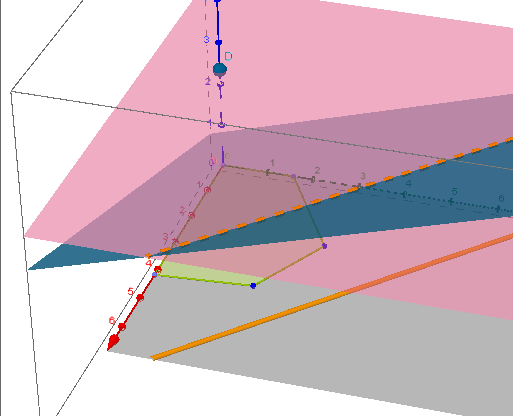
\includegraphics[width=.9\linewidth]{imagen.png}
\end{center}
\end{frame}

\begin{frame}[label={sec:org10d6c49}]{Ejemplos}
\begin{itemize}
\item El problema de la dieta.
\item Optimización de lugares en una excursión.
\item Escoger objetos optimos para un campamento.
\item El problema del flujo máximo.
\end{itemize}
\end{frame}


\begin{frame}[label={sec:orgbac08ff}]{Convexidad.}
Un conjunto \(X\) es \alert{convexo} si para todos \(x,y\in X\) y \(t\in [0,1]\) se tiene que  \(tx+(1-t)y\in X\).
\end{frame}





\begin{frame}[label={sec:orgccb76cb}]{Método símplex}
\end{frame}
\begin{frame}[label={sec:org60fe1e9}]{Método grafico}
\end{frame}


\section{Herramientas computacionales}
\label{sec:org429300f}

\begin{frame}[label={sec:orgae1a31e}]{Emacs}
\begin{center}
\begin{tabular}{ll}
C-x C-s & salvar archivo\\
C-x C-f & abrir archivo\\
M-q & Formatear párrafo\\
C-x d & Editar directorios\\
C-g & Interrumpe\\
C-x1 & Cierra una ventana\\
C-x2 & Divide horizontalmente\\
C-x3 & Divide veticalemte\\
M-w & Copiar\\
C-e & borrar\\
Shift-fechas & Seleccionar region\\
C-y & Pegar la región\\
 & \\
\end{tabular}
\end{center}
\end{frame}

\begin{frame}[label={sec:org2512f9b}]{Git}
\begin{block}{Github}
\end{block}
\begin{block}{Git en la terminal}
\end{block}
\end{frame}

\begin{frame}[label={sec:org204818b}]{Python}
\begin{block}{Jupyter}
\end{block}
\begin{block}{Lenguaje  Python}
\end{block}
\end{frame}

\begin{frame}[label={sec:org9250dbc}]{LaTex}
\end{frame}
\end{document}